\documentclass[twocolumn, fontsize=10pt]{article}
\usepackage[margin=0.70in]{geometry}
\usepackage{lipsum,mwe,abstract}
\usepackage[english]{babel} 
\usepackage{fancyhdr} % Custom headers and footers
\pagestyle{fancyplain} % Makes all pages in the document conform to the custom headers and footers
\fancyhead{} 
\fancyfoot[C]{\thepage} % Page numbering for right footer
\setlength\parindent{0pt} 
\usepackage{amsmath,amsfonts,amsthm} % Math packages
\usepackage{wrapfig}
\usepackage{graphicx}
\usepackage{float}
\usepackage{subcaption}
\usepackage{comment}
\usepackage{enumitem}
\usepackage{makeidx}
\makeindex
\usepackage{cuted}
\usepackage{sectsty} % Allows customizing section commands
\usepackage{xcolor} % For colored text
\usepackage{hyperref} % Package for links
\hypersetup{
    colorlinks=true,
    linkcolor=blue,
    filecolor=magenta,      
    urlcolor=blue,
    }
\allsectionsfont{\normalfont \normalsize \scshape} % Section names in small caps and normal fonts

\addto\captionsenglish{\renewcommand{\contentsname}{Índice}}

\renewenvironment{abstract} % Change how the abstract look to remove margins
 {\small
  \begin{center}
  \bfseries Resumen \vspace{-.5em}\vspace{0pt}
  \end{center}
  \list{}{%
    \setlength{\leftmargin}{0mm}
    \setlength{\rightmargin}{\leftmargin}%
  }
  \item\relax}
 {\endlist}

 \newenvironment{englishabstract} % Abstract en inglés
 {\small
  \begin{center}
  \bfseries Abstract \vspace{-.5em}\vspace{0pt}
  \end{center}
  \list{}{%
    \setlength{\leftmargin}{0mm}
    \setlength{\rightmargin}{\leftmargin}%
  }
  \item\relax}
 {\endlist}
 
\makeatletter
\renewcommand{\maketitle}{\bgroup\setlength{\parindent}{0pt} % Change how the title looks like
\begin{flushleft}
  \begin{center}
    {\color{black} \Large Facultad de Matemática y Computación. Universidad de La Habana. \\
    \color{black} Inteligencia Artificial y Simulación. \\ \vspace{10pt}}
    \href{https://github.com/DanielMPMatCom/AI-Simulation-Project-2024.git}{Repositorio del Proyecto en GitHub} % Add GitHub link here
    \vspace{10pt}
  \end{center}
  \textbf{\@title}
  \@author \\ 
  \@date
\end{flushleft}\egroup
}
\makeatother

%% ------------------------------------------------------------------- 

\title{

\Large Simulación de un Sistema Eléctrico basado en Plantas Termoeléctricas.  \\
[10pt] 
}
\date{\today}
\author{Daniel Machado Pérez - daniel.machado.0206@gmail.com \\
Daniel Toledo Martínez - daniel020126@gmail.com \\
Osvaldo R. Moreno Prieto - osvaldo020213@gmail.com}

\begin{document}

\twocolumn[ \maketitle ]



% --------------- ABSTRACT
\begin{abstract}
    Este proyecto se centra en la simulación de un sistema de plantas termoeléctricas
    que abastecen de energía a varios circuitos distribuidos en una región geográfica.
    Se implementa un generador de un mapa del sistema, ubicando circuitos, termoeléctricas
    y una línea principal a la que se conectan todos los componentes y por la que pasa toda
    la energía producida. Cada termoeléctrica cuenta con varias partes o piezas que garantizan
    su funcionamiento, y un agente planificador con arquitectura BDI que se encarga de tomar decisiones
    sobre el régimen de mantenimientos y reparaciones a las piezas. Cada circuito consta de uno o más bloques 
    que lo dividen y reciben electricidad por separado. Por último existe un agente superior que simula
    al Jefe de la Empresa Eléctrica y toma decisiones con respecto a la distribución óptima de electricidad, 
    también con arquitectura BDI. Para garantizar la efectividad de las decisiones se utiliazn
    componentes de Búsqueda, Conocimiento y Procesamiento de Lenguaje Natural.

\end{abstract}

\begin{englishabstract}
  This project focuses on the simulation of a system of thermoelectric plants that supply energy to various circuits distributed across a geographical region. A system map generator is implemented, placing circuits, thermoelectric plants, and a main power line connecting all components, through which all produced energy flows. Each thermoelectric plant consists of several parts that ensure its proper functioning, and a BDI (Belief-Desire-Intention) architecture planning agent is responsible for making decisions regarding the maintenance and repair schedule of these parts. Each circuit is divided into one or more blocks, which receive electricity separately. Additionally, there is a higher-level agent simulating the Chief of the Electric Company, who makes decisions regarding the optimal distribution of electricity, also based on a BDI architecture. To ensure the effectiveness of decision-making, components from the fields of Search, Knowledge Representation, and Natural Language Processing, within Artificial Intelligence, are utilized.
\end{englishabstract}

\rule{\linewidth}{0.5pt}

% --------------- KEYWORDS
\noindent \textbf{Palabras Clave}: Termoeléctrica, Circuito, Bloque, Caldera, Generador, 
Turbina de vapor, Serpentines, Agente, BDI, Belief, Desire, Intention, Algoritmo Genético (GA), 
Lógica Difusa, Modelo Extenso de Lenguaje (LLM)



% --------------- MAIN CONTENT

\tableofcontents

\section{Introducción}

En esta sección estaremos definiendo el problema en cuestión, 
sus componentes (que serán abordadas a detalle más adelante),
los objetivos planteados y algunas cuestiones técnicas que
forman parte del marco teórico sobre el que se sustenta la investigación.

\subsection{Descripción del Proyecto}

El \textbf{Sistema Eléctrico} que se consideró consta de un conjunto de \textbf{Plantas Termoeléctricas}
situadas relativamente cercanas a un conjunto de circuitos distribuidos en un mapa 2D.
Se asume que cada termoeléctrica consta de 4 tipos de piezas principales:
\textbf{Calderas}, \textbf{Turbina de Vapor}, \textbf{Serpentines}, \textbf{Generador} \cite{parts}.
En este proyecto se decidió abstraerse de la función que cumple cada una de estas piezas
en una verdadera Planta Termoeléctrica. En cambio se otorgó relevancia a la implicación de
una rotura de cada una de ellas en el rendimiento de la termoeléctrica. Se asumió que una planta
 puede tener una o más calderas, y que la generación de la planta está dividida en cada una de sus calderas,
 es decir, al romperse una caldera se pierde la generación que corresponde a la capacidad máxima entre el total
 de calderas. Eso quiere decir que si dejan de funcionar todas las calderas al mismo tiempo la planta no producirá energía.
 En cuanto a las demás partes, cada planta posee una sola de cada una de ellas y su rotura implica la salida de circulación
 de la termoeléctrica del sistema eléctrico. Cada termoeléctrica tendrá una generación máxima, una ubicación en el mapa,
 una planilla del costo de suministrar energía a cada circuito, una energía almacenada y un \textbf{Agente} planificador de
 mantenimientos y reparaciones a sus partes.\\
 Los \textbf{Circuitos} fueron modelados como un conjunto de \textbf{Bloques}, un consumo eléctrico por hora, 
 un nivel de industrialización y una cantidad de ciudadanos. Cada uno tiene una ubicación en el mapa inicial y está conectado 
 a la línea principal de la red eléctrica. Cada bloque consta de una demanda energética, un registro de los horarios de corte 
 eléctrico, y una opinión general de sus habitantes sobre el servicio de la Empresa Eléctrica, obtenido con la ayuda de la \textbf{Lógica Difusa}. 
 Además tienen un consumo diario por hora, una cantidad de ciudadanos y un nivel de industrialización igual
 al del circuito al que pertenece. La suma de los consumos de los bloques conforman el consumo del circuito. 
 Lo mismo pasa con la cantidad de ciudadanos. Como cada circuito y cada termoeléctrica
 está conectada al sistema energético de toda la región, se cumple que desde cualquier planta se puede suministrar
 energía a cualquier circuito, teniendo en cuenta el costo por la distancia.\\
 Para decidir la distribución de energía en el sistema existe el \textbf{Jefe de la Empresa Eléctrica}, modelado con otro agente
 con arquitectura \textbf{BDI}, que recibe información del estado de las termoeléctricas y los circuitos, dígase generación, demanda, estado de opinión,
 impacto económico, etc, y con la asistencia de componentes de \textbf{Inteligencia Artifical} optimiza la el abastecimiento. Este agente
 tiene la potestad de dejar de suministrar energía a un bloque en determinados horarios, cosa que estará obligado a hacer en el caso de la 
 existencia de déficit.

\subsection{Objetivos}
Se simula el comportamiento del sistema y las interacciones de los agentes buscando una planificación eficiente de la distribución de energía.
Se pretende crear un método que dado cualquier configuración geográfica inicial de un sistema eléctrico, sea capaz de modelar
escenarios donde se manejen los recursos de manera efectiva y se muestre un buen rendimiento relativo a las condiciones con las que se cuentan.  

\subsection{Variables que describen el problema}

Para describir el problema, se necesitan variables que nos permitan representar los siguientes fenómenos:
\begin{itemize}

    \item Tiempo entre roturas de una pieza de una planta termoeléctrica.
    \item Tiempo de reparación de una pieza de una planta termoeléctrica.
    \item Demanda diaria por hora de energía de un circuito.
\end{itemize}
\subsubsection{Tiempo entre roturas de una pieza de una planta termoeléctrica.}
    
Según la literatura, \( Weibull(\alpha, \lambda) \) es una distribución comúnmente utilizada para modelar la distribución de fallos (en sistemas) cuando la tasa de fallos es proporcional a una potencia del tiempo, donde \( \alpha \) es el parámetro de forma y \( \lambda \) es el parámetro de escala de la distribución.
\begin{itemize}
    \item Un valor \( \alpha < 1 \) indica que la tasa de fallos disminuye con el tiempo.
    \item Cuando \( \alpha = 1 \), la tasa de fallos es constante en el tiempo.
    \item Un valor \( \alpha > 1 \) indica que la tasa de fallos aumenta con el tiempo.
\end{itemize}

El parámetro \( \lambda \) es un factor de escala que estira o comprime la distribución. Proporciona una estimación de la "vida característica" del producto, que es el tiempo en el cual el 63.2\% del equipo habrá fallado.

El análisis de Weibull ayuda a predecir el comportamiento futuro de fallos de un componente o sistema. Esta capacidad predictiva ayuda en la planificación de actividades de mantenimiento, reduciendo tiempos de inactividad no planificados y aumentando la eficiencia general del sistema.\\

\textbf{Función de Distribución Acumulada:}\\
$ F(x) = 1 - e^{-(\lambda x)^\alpha} $, para $x > 0 $

Para generar valores con una distribución Weibull, se utilizó su implementación de la biblioteca \textbf{random} de Python.

\subsubsection{Tiempo de reparación de una planta termoeléctrica}


Una distribución log-normal es una distribución de probabilidad de una variable aleatoria cuyo logaritmo está distribuido normalmente. En otras palabras, si una variable \( X \) sigue una distribución log-normal, entonces \( \ln(X) \) sigue una distribución normal. La distribución log-normal es útil para modelar datos positivos que son asimétricos y tienen una cola larga a la derecha, lo que significa que los valores extremos altos son más comunes. \\

Debido a esta característica, dicha distribución se ajusta bien en esta parte del problema, ya que los tiempos de reparación tienden a concentrarse hacia el extremo derecho (mayor) de los datos. \\

\textbf{Propiedades de la Distribución Log-normal:}

\textbf{Definición Matemática:}
Si \( X \) es una variable aleatoria distribuida log-normal, entonces:
\[ X \sim \text{Lognormal}(\mu, \sigma^2) \Rightarrow \ln(X) \sim N(\mu, \sigma^2) \]

Aquí, \( \mu \) y \( \sigma \) son los parámetros de la distribución normal de \( \ln(X) \), donde \( \mu \) es la media y \( \sigma^2 \) es la varianza. \\

\textbf{Función de Densidad de Probabilidad (PDF):}\\
La función de densidad de probabilidad de una distribución log-normal se define como:\\
$ f_X(x) = \frac{1}{x \sigma \sqrt{2 \pi}} e^{\left(-\frac{(\ln(x) - \mu)^2}{2 \sigma^2}\right)} $,  para $x > 0$

\subsubsection{Demanda diaria por hora de energía de un circuito}
El consumo diario de energía de un circuito puede ser modelado con una mezcla de distribuciones 
normales (\textit{Gaussian Mixture}), puesto que en un día común se experimentan 2 picos de consumo 
energético, uno en la mañana aproximadamente de 5:00am a 9:00am y otro mayor en la noche de 5:00pm 
a 9:00pm.
Partiendo de un consumo base y proporcionando como parámetros la variabilidad, desviación estándar, media y peso de cada pico puede obtenerse una distribución del consumo en las 24 horas de un día.\\


\section{Generación del Mapa Inicial}

Para la creación del mapa se implementó un generador que primeramente coloca circuitos en posiciones aleatorias 
de una matriz 2D. Luego utilizando clusterización ubica las $n$ termoeléctricas en los $n$ centroides calculados.
A continuación, utilizando intermpolación primeramente por las termoeléctricas y hasta que no existan puntos aislados se generan las 
\textbf{Torres de Alta Tensión}, que están unidas por segmentos que conforman la línea principal del Sistema Energético. 
Finalmente a través de geometría básica se genera el `cableado' con la menor distancia de cada termoeléctrica y circuito a la línea principal, calculando y guardando dichas distancias en el proceso.

\begin{figure}[h]
  \centering
  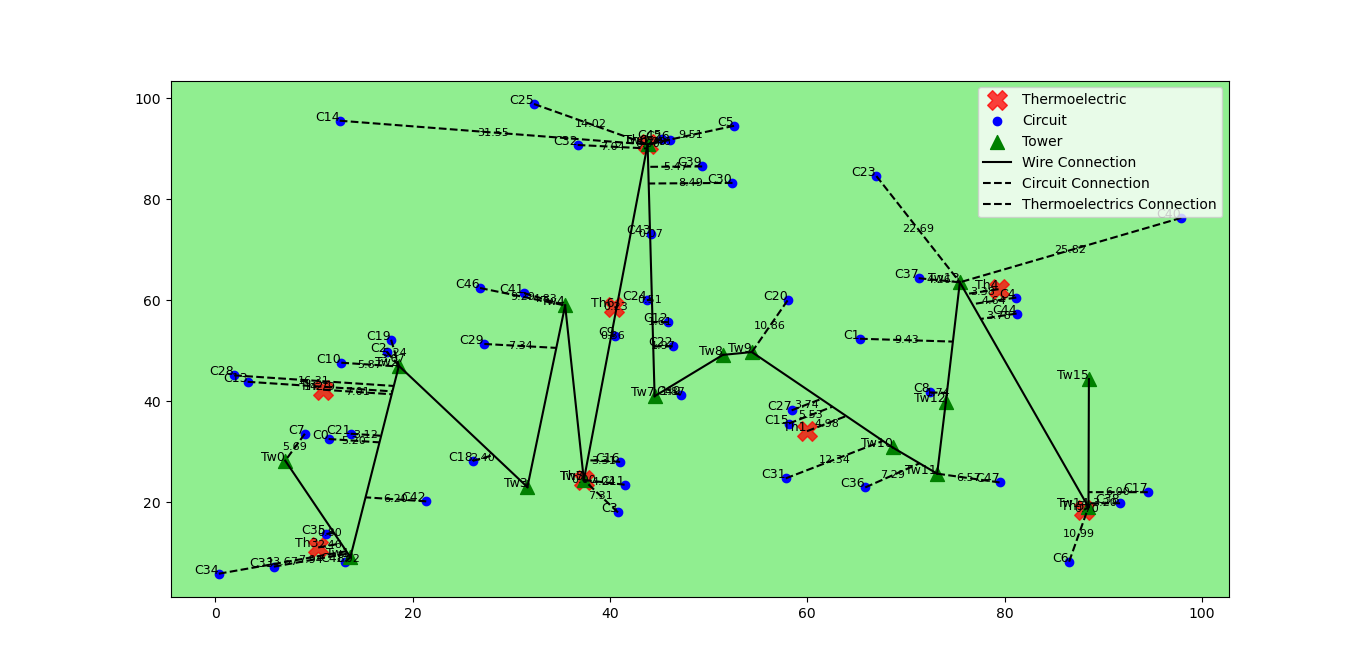
\includegraphics[width=\columnwidth]{assets/map_example.png}
  \caption{Ejemplo de mapa.}
  \label{fig:ejemplo}
\end{figure}

\section{Agentes con Arquitectura BDI}

La arquitectura BDI (Beliefs-Desires-Intentions) en la simulación mediante agentes
les permite modificar su conocimiento del medio o creencias a través del recibimiento
de una percepción, generar nuevas opciones para reformular sus deseos y filtrar las intenciones
que debe tener para llevarlos a cabo, para de esta manera actuar e interactuar para lograr sus objetivos. \cite{book}
En este proyecto fueron utilizados dos tipos de agentes con arquitectura BDI:
\begin{itemize}
  \item \textbf{Agente de Termoeléctrica}: Existe uno en cada Termoeléctrica y sus objetivo es mantenerla funcionando para aportar el mejor rendimiento posible al Sistema Eléctrico.
  \item \textbf{Jefe de la Empresa Eléctrica}: Existe solo uno y se encarga de encontrar y ejecutar la mejor planificación posible de la distribución de energía en dependencia de sus circunstancias en cada momento.
\end{itemize}

\subsection{Agente de Termoeléctrica}
Su percepción se basa en el conocimiento del estado de su 
termoeléctrica y de algunos datos del estado general del 
sistema como la demanda y la oferta del día anterior. 
También puede conocer un tiempo estimado de rotura de las 
piezas de la termoeléctrica, lo cual serviría para planificar 
posibles mantenimientos, su máxima generación posible, su generación actual y
la pérdida de capacidad de generación ante la rotura de una pieza.
\subsubsection{Beliefs}

\begin{itemize}
  \item \textbf{plant\_is\_working}: True si la Planta Termoeléctrica del Agente está funcionando, False en caso contrario.
  \item \textbf{parts\_status}: Una lista de tuplas con 3 elementos, donde el primer elemento es la instancia de la parte, el segundo es True si la parte está funcionando y False en caso contrario, y el tercer elemento indica el tiempo de vida útil estimado restante.
  \item \textbf{broken\_parts}: Una lista de partes que están actualmente rotas.
  \item \textbf{max\_capacity}: La capacidad máxima de la Planta Termoeléctrica.
  \item \textbf{current\_capacity}: La capacidad actual de la Planta Termoeléctrica.
  \item \textbf{power\_output\_reduction\_on\_part\_failure}: Una lista de tuplas donde el primer elemento es la Parte y el segundo es la reducción de producción de energía cuando falla.
  \item \textbf{general\_deficit}: El déficit general del Sistema Eléctrico.
  \item \textbf{general\_demand}: La demanda general del Sistema Eléctrico.
  \item \textbf{general\_offer}: La oferta general del Sistema Eléctrico.
  \item \textbf{all\_desires}: Todos los deseos posibles del Agente.
  \item \textbf{current\_desires}: Los deseos actuales del Agente.
\end{itemize}
\subsubsection{Desires}
\begin{itemize}
  
  \item \textbf{maintain\_maximum\_power\_output}: Deseo de mantener la máxima producción de energía. (True o False)
  \item \textbf{prevent\_unexpected\_breakdowns}: Deseo de prevenir fallos inesperados. (True o False)
  \item \textbf{minimize\_downtime}: Deseo de minimizar el tiempo de inactividad. (True o False)
  \item \textbf{meet\_energy\_demand}: Deseo de satisfacer la demanda de energía. (True o False)
  \item \textbf{prioritize\_critical\_part\_repair}: Deseo de priorizar la reparación de partes críticas. (True o False)
  \item \textbf{repair\_parts}: Deseo de reparar las partes dañadas. Es una lista de tuplas en la que cada tupla contiene una parte de la planta termoeléctrica y un valor booleano que indica si esa parte necesita ser reparada o no.

\end{itemize}

\subsubsection{Intentions}

\begin{itemize}
  \item \textbf{increase\_power\_output}: Intención de aumentar la producción de energía
  \item \textbf{operate\_at\_full\_capacity}: Intención de operar a plena capacidad
  \item \textbf{perform\_maintenance\_on\_parts}: Una lista de tuplas donde el lado izquierdo es la Parte y el lado derecho es Verdadero si la Parte necesita mantenimiento
  \item \textbf{reduce\_downtime}: Intención de reducir el tiempo de inactividad
  \item \textbf{prioritize\_repair\_of\_critical\_parts}: Intención de priorizar la reparación de partes críticas
  \item \textbf{repair\_parts}: Una lista de tuplas donde el lado izquierdo es una Parte y el lado derecho es Verdadero si hay intención de reparar la parte y Falso en caso contrario

\end{itemize}

\subsection{Jefe de la Empresa Eléctrica}

\subsubsection{Beliefs}

\subsubsection{Desires}
\subsubsection{Intentions}

\section{Algoritmo Genético}

\section{Lógica Difusa}

\section{Modelo Extenso de Lenguaje}

\section{Ejecución de la Simulación}

\section{Resultados y Estadísticas}

\section{Conclusiones}


\renewcommand\refname{Referencias}

\begin{thebibliography}{}

  \sloppypar
  \bibitem{parts} Fundación Endesa. (s.f.). Central térmica convencional. Fundación Endesa. \url{https://www.fundacionendesa.org/es/educacion/endesa-educa/recursos/centrales-electricas-convencionales/central-termica-convencional}


  \bibitem{book} García Garrido, L., Martí Orosa \& L., Pérez Sánchez, L. (n.d.) Temas de Simulación. [Publisher not identified]

\end{thebibliography}
    
    

\end{document}
